\subsubsection{Iteratoren}

\begin{frame}{Iteratoren}
    Der Begriff \emph{Iterator} stammt aus dem Bereich der Softwareentwicklung und bezeichnet einen Zeiger, mit dem die Elemente einer Menge durchlaufen werden können (z. B. eine Liste, ein Vector etc.).
\end{frame}

\begin{frame}[fragile]{Beispiel - Beispiel (Code)}
    \begin{minted}{cpp}
std::vector<int> v{ 3, 1, 4, 1, 5, ... };

for (std::vector<int>::iterator it = v.begin();
    it != v.end(); ++it)
    std::cout << *it << ", ";

std::cout << std::endl;

// 3, 1, 4, 5, 1, ...,
    \end{minted}
\end{frame}

\begin{frame}[fragile]{Iteratoren - Beispiel (Graphisch)}
    \begin{minted}{cpp}
std::vector<int>::iterator it = v.begin();
    \end{minted}

    \begin{center}
        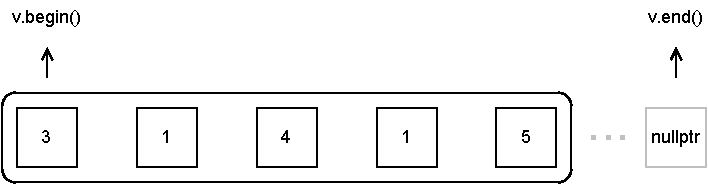
\includegraphics[width=0.75\textwidth]{pictures/iterators_example_1.pdf}
    \end{center}
\end{frame}

\begin{frame}[fragile]{Iteratoren - Beispiel (Graphisch)}
    \begin{minted}{cpp}
std::cout << *it << ", ";
    \end{minted}

    \begin{center}
        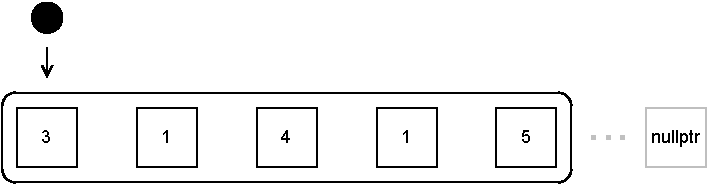
\includegraphics[width=0.75\textwidth]{pictures/iterators_example_2.pdf}
    \end{center}
\end{frame}

\begin{frame}[fragile]{Iteratoren - Beispiel (Graphisch)}
    \begin{minted}{cpp}
++it;
    \end{minted}

    \begin{center}
        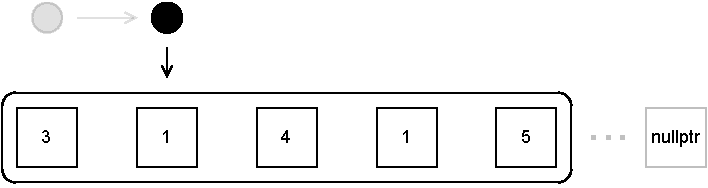
\includegraphics[width=0.75\textwidth]{pictures/iterators_example_3.pdf}
    \end{center}
\end{frame}

\begin{frame}[fragile]{Iteratoren - Beispiel (Graphisch)}
    \begin{minted}{cpp}
it == v.end();
    \end{minted}

    \begin{center}
        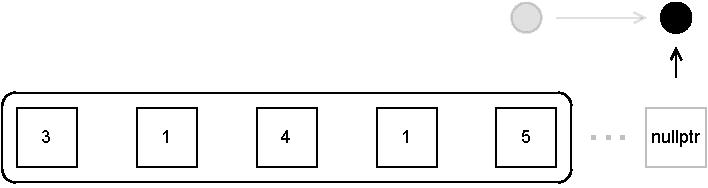
\includegraphics[width=0.75\textwidth]{pictures/iterators_example_4.pdf}
    \end{center}
\end{frame}